\documentclass[10pt, a4paper]{article}
\usepackage[utf8]{inputenc}
\usepackage[paper=a4paper, left=1.5cm, right=1.5cm, bottom=1.5cm, top=3.5cm]{geometry}
\usepackage[spanish]{babel}
\usepackage{indentfirst}
\usepackage{fancyhdr}
\usepackage{latexsym}
\usepackage{lastpage}
\usepackage[colorlinks=true, linkcolor=blue]{hyperref}
\usepackage{calc}
\usepackage{verbatim}
\usepackage{listings}
\usepackage{amsfonts}
\usepackage{float}
\setcounter{tocdepth}{5}
\usepackage{caption}
\usepackage{subcaption}
\sloppy

\parskip=5pt % 10pt es el tamaño de fuente

% Pongo en 0 la distancia extra entre ítemes.
\let\olditemize\itemize
\def\itemize{\olditemize\itemsep=0pt}

\usepackage{caratula}

% Acomodo fancyhdr.
\pagestyle{fancy}
\thispagestyle{fancy}
\addtolength{\headheight}{1pt}
\lhead{S. Aboy Solanes, E. Almansi, F. Canay, F. Decroix}
\rhead{$2^{\mathrm{do}}$ cuatrimestre de 2014}
\cfoot{\thepage /\pageref{LastPage}}
\rfoot{Trabajo Práctico 1 - Wiretapping}
\renewcommand{\footrulewidth}{0.4pt}

\begin{document}


\titulo{Trabajo Práctico 1 - Wiretapping}
\fecha{Martes 23 de Septiembre}
\materia{Teoría de las Comunicaciones}
\integrante{Saboy Solanes}{175/12}{santiaboy2@hotmail.com}
\integrante{Emilio Almansi}{674/12}{ealmansi@gmail.com}
\integrante{Federico Canay}{250/12}{fcanay@hotmail.com}
\integrante{Facundo Decroix}{842/11}{fndecroix92@hotmail.com}

%Pagina de titulo e indice
\thispagestyle{empty}

\maketitle

%\thispagestyle{empty}
%\mbox{}
%\newpage
\thispagestyle{empty}
\tableofcontents

\newpage

\section{Introducción}
En este trabajo práctico vamos a abordar el desarrollo de herramientas de diagnóstico de red. Nuestro objetivo va a ser analizar estadísticamente el protocolo ARP. Por otro lado, vamos a sacar conclusiones acerca de los tipos de dispositivos de red que se pueden encontrar en un segumento de red determinado. Para ello, utilizamos la herramienta de manipulación y análisis de paquetes, Scapy.

\section{Desarrollo}
Antes de comenzar el desarrollo vamos a definir algunos términos.

$\bullet$ \textbf{Informacion}: Dado un evento E decimos que cuando E tiene lugar, recibimos
\begin{center}
$I (E) = log(\frac{1}{P(E)})$ 
\end{center}

unidades de información. Al usar $log_2$ la unidad obtenida es bits.

$\bullet$ \textbf{Entropía}: La entropía de un mensaje X, que se representa por H(X), es el valor medio ponderado de la cantidad de información de los diversos estados del mensaje 

\begin{center}
$H(X) = - \Sigma$ $p(x)$ $log$ $p(x)$
\end{center}

$\bullet$ \textbf{Nodo distinguido}: En una fuente, un nodo distinguido es un nodo cuya información es menor a la entropía de dicha fuente.

\subsection{Capturando tráfico}
Para el desarrollo de este trabajo práctico escuchamos pasivamente redes para poder observar que sucedía en las mismas. En particular, capturamos paquetes ARP \emph{who-has}.

Utilizamos dos modelos de fuente de información:

$S_{dst}$ = \{$s_1$ $\cdots$ $s_n$\} siendo $s_i$ una IP que aparece como dirección destino en los paquetes ARP \emph{who-has}

$S_{src}$ = \{$s_1$ $\cdots$ $s_n$\} siendo $s_i$ una IP que aparece como dirección origen en los paquetes ARP \emph{who-has}

Creamos una \emph{tool} que escucha pasivamente en la red local. Luego, la adaptamos para que estime las probabilidades de dichas fuentes en función de los paquetes ARP observados y que calcule la entropía de las mismas.

Usando dicha herramienta, realizamos capturas de paquetes ARP sobre distintas LANs: Alto Palermo, Red laboral de Honeywell, Laboratorios de Ciudad Universitaria (Via Wi-Fi), y la casa de un integrante del grupo.

\subsection{Gráficos y análisis}
Una vez que capturamos el tráfico, nos propusimos gráficar y a analizar los datos obtenidos. Graficamos en forma de histogramas, y de grafos la información y entropía de $S_{dst}$ y $S_{src}$.

$\bullet$ Experimento ``Red Hogareña''

Capturamos el tráfico de la LAN de un integrante de nuestro grupo. A continuación presentamos un grafo que muestra el pasaje de paquetes ARP entre las distintas IPs.

\begin{figure}[H]
  \begin{center}
    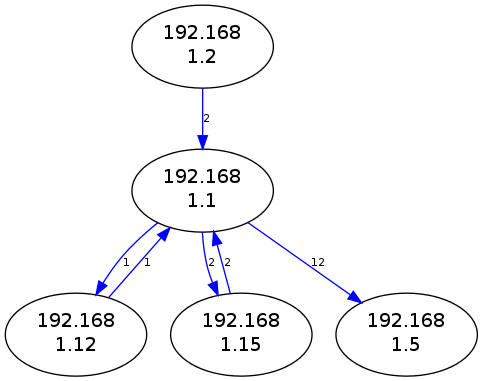
\includegraphics[width=\linewidth/2]{../imgs/pruebaFede-ips_red.png}
    \label{fig:FedeGrafo}
    \caption{Grafo de LAN hogareña}
  \end{center}
\end{figure}


 % \begin{figure}[H]
 %   \begin{minipage}{0.5\linewidth}
 %     \includegraphics[width=\linewidth]{graficos/goloso_tiempo.eps}
 %     \caption{Tiempo ejecución goloso}\label{fig:goloso-tiempo}
 %   \end{minipage}
 %  \hfill
 %   \begin{minipage}{0.5\linewidth}
 %     \includegraphics[width=\linewidth]{graficos/goloso_tiempo_div_n.eps}
 %     \caption{Tiempo de goloso dividido n}\label{fig:goloso-tiempo-n}
 %   \end{minipage}
 % \end{figure}



\section{Resultados}

\subsection{Red Alto Palermo}

\subsubsection{Descripción}

lugar, dia de la semana, hora aproximada, fecha, wifi o ethernet
cantidad de paquetes tomados, tiempo de muestreo

\subsubsection{Topología de la red}

grafico del grafo de la red

\subsubsection{Fuente: $S_{dst}$}

histograma
grafico de informacion
entropía total

\subsubsection{Fuente: $S_{src}$}

histograma
grafico de informacion
entropía total

\subsection{Red Honeywell}

\subsubsection{Descripción}

lugar, dia de la semana, hora aproximada, fecha, wifi o ethernet
cantidad de paquetes tomados, tiempo de muestreo

\subsubsection{Topología de la red}

grafico del grafo de la red

\subsubsection{Fuente: $S_{dst}$}

histograma
grafico de informacion
entropía total

\subsubsection{Fuente: $S_{src}$}

histograma
grafico de informacion
entropía total

\subsection{Red Laboratorios DC}

\subsubsection{Descripción}

lugar, dia de la semana, hora aproximada, fecha, wifi o ethernet
cantidad de paquetes tomados, tiempo de muestreo

\subsubsection{Topología de la red}

grafico del grafo de la red

\subsubsection{Fuente: $S_{dst}$}

histograma
grafico de informacion
entropía total

\subsubsection{Fuente: $S_{src}$}

histograma
grafico de informacion
entropía total

\subsection{Red hogareña}

\subsubsection{Descripción}

lugar, dia de la semana, hora aproximada, fecha, wifi o ethernet
cantidad de paquetes tomados, tiempo de muestreo

\subsubsection{Topología de la red}

grafico del grafo de la red

\subsubsection{Fuente: $S_{dst}$}

histograma
grafico de informacion
entropía total

\subsubsection{Fuente: $S_{src}$}

histograma
grafico de informacion
entropía total

\section{Discusión general}

\section{Conclusión}
Como conclusión, queremos recalcar que por lo general los routers son nodos distinguidos en las LANs a las que pertenecen. Esto se mantiene, ya sea una red pública o privada.

Como pudimos ver en los experimentos, creemos que es importante saber que esto no necesariamente siempre es así. En el caso de Ciudad Universitaria, el servidor local era un nodo distinguido.

Para finalizar, en este trabajo práctico aprendimos que LA AMISTAD RESUELVE TODOS LOS PROBLEMAS.
\end{document}	